\section{Computing error in specific observables}
\label{sec:specific}

\subsection{Basics}
``What error bar should I report?''
Here we address this simple but critical question.

In general, there is no one-best practice for choosing error bars. However, in the context of simulations, we can nonetheless identify common goals when reporting such estimates: (i) to help authors and readers better understand uncertainty in data; and (ii) to provide readers with realistic information about the reproducibility of a given result.

With this in mind, we recommend the following: (a) in fields where there is a definitive standard for reporting uncertainty, the authors should follow existing conventions; (b) otherwise, such as for biomolecular simulations, \emph{authors should report (and graph) their best estimates of 95\% confidence intervals.} As explained in the glossary above, a 95~\% \hyperref[def:conf_int]{confidence interval} is a range of values that is expected to bracket 95~\% of the computed predictions \emph{if statistically equivalent simulations are repeated a large number of times;} (c) when feasible and especially for a small number of independent measurements ($n < 10$), authors should consider plotting all of the points or a histogram instead of an average with error bars.

We emphasize that as opposed to standard uncertainties [$\stdevmean{\mean{x}}$], confidence intervals have several practical benefits that justify their usage. In particular, they directly quantify the statistical frequency with which we expect a given outcome, which is more relatable to everyday experience than moments of a probability distribution. As such, confidence intervals can help authors and readers better understand the implications of an uncertainty analysis. Moreover, downstream users/readers of a given paper may include less statistically-oriented readers for whom confidence intervals are a more meaningful measure of variation.

In a related vein, error bars expressed in integer multiples of $\stdevmean{\mean{x}}$ can be misinterpreted as unrealistically under or overestimating uncertainty if taken at face value. For example, reporting $3\stdevmean{\mean{x}}$ uncertainties for a normal random variable amounts to a 99.7~\% confidence interval, which is likely to be a significant overestimate for many applications. On the other hand, $1\stdevmean{\mean{x}}$ uncertainties only correspond to a 68~\% confidence interval, which may be too low. Given that many readers may not take the time to make such conversions in their heads, we feel that it is safest for modelers to explicitly state the confidence level of their error bar or reported confidence interval.

In recommending 95~\% confidence intervals, we are admittedly attempting to address a social issue that nevertheless has important implications for science as a whole. In particular, the authors of a study and the reputation of their field do not benefit in the long run by under-representing uncertainty, since this may lead to incorrect conclusions. But perhaps just as importantly, many of the same problems can arise if uncertainties are reported in a technically correct but obscure and difficult-to-interpret manner. For example, $1\stdevmean{\mean{x}}$ error bars may not overlap and thereby mask the inability to statistically distinguish two quantities, since the corresponding confidence intervals are only 68~\%. With this in mind, we therefore wish to emphasize that visual impressions conveyed by figures in a paper are of primary importance. Regardless of what a research paper may explain carefully in text, error bars on graphs create a lasting impression and must be as informative and accurate as possible. If 95~\% confidence intervals are reported, the expert reader can easily estimate the smaller standard uncertainty (especially if it is noted in the text), but showing a graph with overly small error bars is bound to mislead most readers -- even experts who do not search out the fine print.






%We frequently perform molecular simulations to make quantitative estimates of quantities like pressure, free energy or yield strain.  When reporting these estimates, it is important to also provide an estimate of the uncertainty of the result, typically as a standard error.

%A 90\% confidence interval, as explained in the glossary above, is a range of values which is expected to bracket 90\% of the observable values \emph{if the identical simulation is repeated a large number of times.}  Of course, the interval is estimated based on a single simulation, and so it is only approximate; nevertheless, as explained below, there are statistically sound means for estimating the interval from a single simulation.  If additional simulations are performed and used to estimate the confidence interval, one is then trying to estimate the confidence interval for the set of simulations -- and the corresponding interval should be smaller, in general, than that for a single simulation.

%\begin{table}
    %\begin{tabular}{S S}
      %\toprule
       %{Pressure (MPa)} & {Density (mol/L)} \\
      %0.001 & 3.007(3)e-4 \\
      %0.010 & 0.003011(2) \\
      %0.100 & 0.03039(16) \\
      %1.000 & 52.1(5) \\
      %\bottomrule
    %\end{tabular}
  %\caption{Density as a function of pressure for water at a temperature of 400K}
  %\label{tab:uncertainties}
%\end{table}

%[DMZ: SHOULD WE INCLUDE THIS (AND TABLE) GIVEN THAT IT SEEMS FIELD-SPECIFIC?  IF SO, WE SHOULD BE SPECIFIC ABOUT WHICH FIELDS USE THIS CONVENTION - CERTAINLY NOT BIOMOLECULAR SIMULATION.]
As a final note, we remind readers that only significant figures should be reported.
Additional figures beyond the precision implicit in the uncertainty are unhelpful at best, and potentially misleading to readers who may not be aware of the limitations of simulations or statistical analyses generally.
%When reporting quantities with uncertainties, only the digits that are significant should be included and the standard error should be placed after the value in parenthesis as the uncertainty in the last digit.  In general only one digit of uncertainty need be reported unless the digit is 1, in which case, it is helpful to report two digits (in order to avoid up to 50~\% roundoff error in the uncertainty).  See the \TABLE{uncertainties} for examples from hypothetical isobaric simulations of water.


\subsection{Overview of procedures for computing a confidence interval}
We remind readers that before attempting to quantify uncertainty via an error bar, the semi-quantitative checks on sampling (Sec.\ \ref{sec:quick}) should be performed.
If the observable of interest is not fluctuating about a mean value but largely increasing or decreasing during the course of a simulation, it is unlikely that a reliable quantitative estimate for the observable (or an error bar) can be obtained.

For observables passing the qualitative tests noted above in Sec.\ \ref{sec:quick}, we advocate obtaining confidence intervals in one of two ways:
\begin{itemize}
\item For observables that are approximately Gaussian-distributed (or assumed to be, due to lack of information), an appropriately chosen \emph{coverage factor} $k$ (typically about 2, but see Sec.~\ref{sec:conf_int}) multiplying the standard uncertainty $\stdevmean{\mean{x}}$ by $k$ yields an estimate for a 95~\% confidence interval.
\item For non-Gaussian observables, a \emph{bootstrapping} approach (described below) should be used.  An example of a potentially non-Gaussian observable is a rate-constant, which must be positive but could exhibit significant variance, so a confidence interval estimated with a coverage factor may lead to an unphysical negative lower limit.  Multimodal distributions certainly are not Gaussian.  Bootstrapping does not assume an underlying distribution but instead constructs a confidence interval based on the recorded data values, and the limits cannot fall outside the extreme data values.  Bootstrapping (or block averaging) is also necessary for cases for \hyperref[def:deriv_obs]{derived observables}; this is true for quantities such as time correlation functions and anything derived from them.
\end{itemize}

%The standard error is the standard deviation of the distribution of the results that would be obtained by repeating the simulation.  Several techniques to estimate the uncertainty are described below with varying levels of complexity and robustness.  Ultimately, a technique is robust if it can produce an uncertainty estimate that is consistent with the standard deviation of results from actually repeating the simulation and analysis of the data.

Below we describe approaches for estimating the standard uncertainty $\stdevmean{\mean{x}}$ from a single trajectory with a coverage factor $k$ as well as the bootstrapping approach for direct confidence-interval estimation. Whether using a coverage factor and standard uncertainty or bootstrapping, one requires an estimate for the independent number of observations in a given simulation.  This requires care, but may be accomplished based on the effective sample size described in Sec.\ \ref{sec:global}, via block averaging, or by analysis of a time-correlation function. However, these methods have their limitations and must be used with caution.  Primarily, they require the user to look at the correct quantity in order to produce the correct answer.  Both block averaging and autocorrelation analysis will produce different effective sample sizes for different quantities; to produce robust answers, one must identify and track the slowest relevant degree of freedom in the system, which can be a non-trivial task.  Even apparently fast-varying properties may have significant statistical error if they are coupled to slower varying ones, and this error in uncertainty estimation may not be readily identifiable by solely examining the fast-varying time series.

In the absence of a reliable estimate for the number of independent observations, one can perform $n$ independent simulations and calculate the standard deviation $\stdev{x_j}$ for quantity $x$ (which could be the ensemble average of a raw data output or a derived observable) among the $n$ simulations, yielding a standard uncertainty of $\stdevmean{\mean{x}} = \stdev{x_j} / \sqrt{n}$.  When computing the uncertainty with this approach, it is important to ensure that each starting configuration is also independent or else to recognize and report that the uncertainty refers to simulations started from a particular configuration.  The means to obtain independent starting configurations is system-dependent, but might involve repeating the protocol used to construct a configuration (solvating a protein, inserting liquid molecules in a box, etc.), using a new random seed.  However, readers are cautioned that \emph{for complex systems, it may be effectively impossible to generate truly independent starting configurations pertinent to the ensemble of interest.}  For example, a simulation of a protein in water will nearly always start from the experimental structure, which introduces some correlation in the resulting simulations even when the remaining simulation components (water, salt, etc) are regenerated {\it de novo}.

%\subsection{Assessing qualitative behavior of data}

%[DMZ: moved to QUICK-AND-DIRTY SECTION

%Generally speaking, analysis routines that extract derived quantities from raw data are often formulated on the basis of physical intuition about how that data should behave.  Before proceeding to data analysis, it is therefore useful to assess the extent to which raw data conforms to these expectations and the requirements imposed by either the modeler or the analysis routines.  Such tasks help reduce subjectivity of predictions and offer insight into when a simulation protocol should be revisited to better understand their meaningfulness \cite{patrone1}.  Unfortunately, general recipes for assessing data quality are impossible to formulate, owing to the range of physical quantities of interest to modelers.  Nonetheless, a short example will help clarify the matter.

%In the context of materials science, understanding when a structural material fails is critical for many engineering applications.  In the past decade, scientists have increasingly focused on modeling the yield-strain $\epsilon_y$, which is (loosely speaking) the amount of stretching (or strain) at which it deforms irreversibly.  Intuition and experiments tells us that upon deforming a material by a fraction $1+\epsilon$, it should recover its original dimensions if $\epsilon \le \epsilon_y$ and have a residual strain $\epsilon_r = \epsilon - \epsilon_y$ if $\epsilon \ge \epsilon_y$ \cite{patrone2}.  Owing to the time-scale limitations of MD, it is also reasonable to expect that the transition in $\epsilon_r$ around yield will be smooth and not piecewise linear.  Thus, if we fit residual strain to a hyperbola, the proximity of data to the asymptotes illustrates the extent to which simulated $\epsilon_r$ conforms to the expectation that $\epsilon_r=0$ when $\epsilon < \epsilon_y$.  See Fig.~\ref{fig:yield}.

%\begin{figure}
%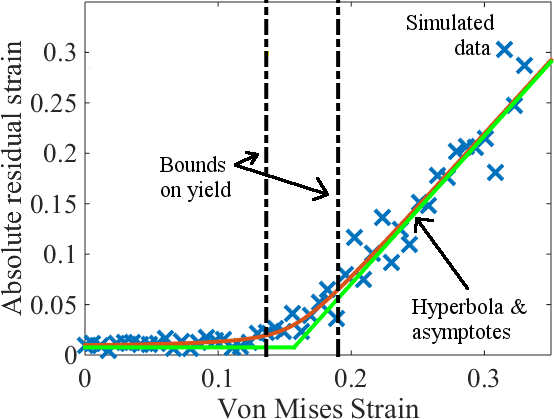
\includegraphics[width=8cm]{hyperbola.png}\caption{Yield strain tn $\epsilon_r$ as a function of applied strain $\epsilon$.  Blue $\times$ denote simulated data, whereas the smooth curve is a hyperbola fit to the data.  The green lines are asymptotes; their intersection can be taken as an estimate of $\epsilon_y$.    Bounds on yield are computed by the synthetic data method discussed in the next section.  {\it From, ``Estimation and uncertainty quantification of yield via strain recovery simulations,'' P.\ Patrone, CAMX 2016 Conference Proceedings.  Reprinted courtesy of the National Institute of Standards and Technology, U.S. Department of Commerce. Not copyrightable in the United States.}}\label{fig:yield}
%\end{figure}

\subsection{Block averaging method for estimating the standard uncertainty}\label{sec:blockavg}

The standard uncertainty of a simulation observable can be estimated from the \hyperref[def:exp_st_dev]{experimental standard deviation} of the observable divided by the square root of the number of independent samples.
Due to correlation in the tape of simulation output from either MD or MC simulation, the number of independent samples in a simulation is neither equal to the number of observations nor known {\it a priori}.
The block averaging technique can be used instead of the individual observations to account for correlation in samples, while using all data, subject only to the constraint that the ``blocks'' are large enough to be essentially uncorrelated\cite{Friedberg1970,Flyvbjerg-1989,FrenkelSmit2002,Grossfield2009}.

Briefly, the set of $N$ observations $\left\{x_1, ..., x_N\right\}$ are converted to a set of $M$ ``block averages'' $\left\{x^b_1, ..., x^b_{M}\right\}$, where a block average $x^b_j$ is the \hyperref[def:arith_mean]{arithmetic mean} of $n$ (the block size) sequential measurements of $x$:
%
\begin{equation}
  x^b_j = \dfrac{\sum\limits_{j=1+(k-1)n}^{kn} x_j}{n}
\end{equation}
%
From this set of block averages, one may then compute the arithmetic mean of the block averages, $\mean{x}^b$, which is an estimator for $\expval{x}$.
(We note that for $mod(N,n)=0$, then $\mean{x}^b = \mean{x}$, as the entire set of $x_j$ is used. This is {\it not} true if $N$ is not evenly divisible by either $M$ or $n$.)
Following, one computes the \hyperref[def:exp_st_dev]{experimental standard deviation} of the block averages, $\stdev{\mean{x}^b}$ using Eq.~\ref{def:exp_st_dev}.
Lastly, the standard uncertainty of $\mean{x}^b$ is just the \hyperref[def:exp_st_dev_mean]{experimental standard deviation of the mean} given the set of $M$ block averages:
%
\begin{equation}
  \stdevmean{\mean{x}^b} = \dfrac{\stdev{x^b_j}}{\sqrt{M}}
\end{equation}
%
This standard uncertainty may then be used to calculate a confidence interval on $\mean{x}^b$.

It is crucial when performing this analysis to do so systematically as a function of block size; as the blocks get longer, the block averages should decorrelate and $\stdevmean{\mean{x}^b}$ should plateau \cite{Flyvbjerg-1989,Grossfield2009}.
Another approach is to measure the block correlation and to use it to improve the selection of the block size and, hence, uncertainty estimate \cite{Kolafa1986}.
We stress that this final step of adjusting the block size and recomputing the block standard uncertainty is absolutely necessary. Otherwise, the blocks may be correlated, yielding an uncertainty that is not meaningful.

\subsection{Autocorrelation method for estimating the standard uncertainty}\label{sec:autocorrelation}

An alternative to the more common block averaging technique is the autocorrelation method for estimating the standard uncertainty of an observable.
The essential objective of this technique is to estimate the number of independent samples in a simulation, via an intermediate function known as the autocorrelation function.
First, given a sequence of observations $\left\{x_1, ..., x_N\right\}$, the autocorrelation function $C$ is computed for a set of lags $j$:
%
\begin{equation}
  C_j = \dfrac{
   \overline{
      \left( x_{k{\color{white}j}}\hspace{-1pt} - \mean{x} \right)
      \left( x_{k+j} - \mean{x} \right)
    }
  }
  {\stdev{x_j}^2}
  \label{def:obs_ACF}
\end{equation}
%
where the denominator is the square of the \hyperref[def:exp_st_dev]{experimental standard deviation} of $x_j$ given by Eq.~\ref{def:exp_st_dev}.
Then, the number of independent samples is estimated by\footnote{The reader should note that both the autocorrelation function (Eq. \ref{def:obs_ACF}) and the number of independent samples (Eq.~\ref{def:Nind}) may be written in different forms\cite{Grossfield2009,Chodera-2016}. Our convention here presents the observations as a list $\left\{x_j\right\}$ in which the time interval (Molecular Dynamics) or trial spacing (Monte Carlo) of adjacent $x_j$ is implicitly fixed. For time-series data, one could alternately write both the observations and autocorrelation function as continuous functions of time, e.g.~$x\left(t\right)$ and $C\left(\tau\right)$ where $\tau$ is the lag time. In that case, $N_{ind}$ is written as a division of the total simulation time by the time integral of $C\left(\tau\right)$\cite{Grossfield2009}.}
%\footnote{{\color{red} Explain why this sum is not the same as the integration over $C$; $C$ is stationary and symmetric, 1 comes from the ``zeroth'' lag, 2 is for symmetry. Actually easy to see this if you do an integral from -infty to +infty by a midpoint integration.}}
%
\begin{equation}
  N_{ind} = \dfrac{N}{1+2 \sum_{i=1}^{N_{lags}} C_j}
  \label{def:Nind}
\end{equation}
%
where $N_{lags}$ is the number of lags for which the $C_j$ was computed.
In practice, one rounds $N_{ind}$ to an integer.
Finally, the standard uncertainty is estimated via
%
\begin{equation}
  \stdevmean{\mean{x}} = \dfrac{\stdev{x_j}}{\sqrt{N_{ind}}}
  \label{def:ACF_std_unc}
\end{equation}
%
We note that the \hyperref[def:exp_st_dev]{experimental standard deviation} of the observable $x$ is used in Eq.~\ref{def:ACF_std_unc} to estimate the uncertainty. Strictly speaking, the standard uncertainty should be estimated using the true standard deviation of $x$ (e.g.\ $\sigma_x$); given that the true standard deviation is unknown, the experimental standard deviation is used in its place as an {\it unbiased estimate} of $\sigma_x$\cite{PatroneAIAA}.

\subsection{Propagation of uncertainty}

The quantities we are most interested in may not be simulation observables.  For instance, the free energy difference between two states might be measured by free energy perturbation, expressed as a function of the average of another quantity \cite{Taylor1997}.
\begin{equation}
\beta \Delta A = -\ln \left< \exp \left(-\beta \Delta U\right) \right>
\end{equation}
Although $\exp(-\beta \Delta U)$ can be measured during the simulation and its uncertainty can be estimated directly using block averages as described above, $\beta \Delta A$ cannot be handled the same way.  If we compute $\beta \Delta A$ for each block, the values will tend to take extremely positive whenever the perturbation does poorly (where $\Delta U$ is consistently large).  In the pathological case, $\Delta U$ might be $\infty$ for every sample in a block and the $\beta \Delta A=-\ln 0$ cannot be computed.


Instead of using block averages for $\beta \Delta A$, its uncertainty can be expressed as a first-order Taylor series expansion
%
\begin{equation}
  \sigma_{\beta \Delta A} = \sigma_{\exp(\beta \Delta U)} / \left< \exp \left(-\beta \Delta U\right) \right>
  \label{eq:propagation_bDA}
\end{equation}
%
Propagation of uncertainty is needed whenever the derived quantity can be expressed as a function of other random observables.  It might also be needed when the derived quantity is of a function of quantities measured in separate simulations, such as $<U(T_2)>-<U(T_1)>$.  If a derived quantity is a function of multiple observables measured within a single simulation, then terms must be included to account for the correlation between those observables.

The Taylor series approach works well in most cases and is easy to use, but does have limitations.  Because this approach is based on a first-order Taylor series, propagation of uncertainty can fail in cases where a non-linear formula is used and the uncertainty is very large or the distribution of input averages is not Gaussian.  For instance, the uncertainty in $\beta \Delta A$ as prescribed by Eq.~\ref{eq:propagation_bDA} cannot exceed unity no matter how short the simulation is or how bad the sampling is.  If there is doubt as to the quality of the computed uncertainty, the uncertainty can be estimated with alternative approaches such as bootstrapping to validate the Taylor series results or to identify an alternative approach that works better.

\subsection{From standard uncertainty to confidence interval for Gaussian variables}\label{sec:conf_int}
Once a standard uncertainty value is obtained for a Gaussian-distributed random variable with mean $\left< x \right>$, and the number of independent samples $n$ has been estimated, the 95~\%-confidence interval $\left[ \mean{x} -k \, \stdevmean{\mean{x}} , \mean{x} +k \, \stdevmean{\mean{x}} \right]$ can be constructed on the basis of an established look-up table (or a statistics software model) for the coverage factor $k$ based on $n$.  The theoretical basis for the table is the ``Student'' or ``$t$'' distribution, which is \emph{not} Gaussian, but governs the behavior of an \emph{average} derived from $n$ independent Gaussian variables  \cite{JCGM:GUM2008}. Table \ref{tab:coveragefactors} lists $k$ for two-sided 95~\% confidence intervals for select values of $n$.

When $n \leq 10$, we recommend showing all data points, as a confidence interval may not be statistically meaningful.

\begin{table}
    \begin{tabular}{S S}
      \toprule
       {$n$ (independent samples)} & {$k$ (coverage factor)} \\
       \hline
      6 & 2.57 \\
      11 & 2.23 \\
      16 & 2.13 \\
      21 &  2.09\\
      26 & 2.06 \\
      51 & 2.01 \\
      101 & 1.98 \\
      \bottomrule
    \end{tabular}
  \caption{Coverage factors $k$ required for a two-sided 95~\% confidence interval for a Gaussian variable \cite{JCGM:GUM2008}.}
  \label{tab:coveragefactors}
\end{table}

As a reminder, multi-modally distributed variables with multiple peaks in their distributions cannot be considered Gaussian random variables.  Variables with a strict upper or lower limit (such as a positive-definite quantity) and long-tailed distributions are also not Gaussian.  These cases should be treated with bootstrapping.

\subsection{Bootstrapping}

%The Taylor series approach may fail in some situations, either because a derived quantity cannot be expressed as a function of the measured simulation data or because the first-order truncation of the series is too severe.
Bootstrapping is an approach to uncertainty estimation that does not assume a particular distribution for the observable of interest or a particular kind of relationship between the observable and variables directly obtained from simulation \cite{Tibshirani1998}.  In nonparametric bootsrapping, new, ``synthetic'' data sets (corresponding to hypothetical simulation runs) are created by drawing $n$ samples (configurations) from the original collection that was generated during the actual run.  The same sample may be selected twice, while others may not be selected at all in a process called ``sampling with replacement.''  In doing so, these synthetic sets will be different even though they all have the same number of samples and draw from the same pool of data.  Having created a new set, the data is analyzed to determine the derived quantity of interest, and this process is repeated to produce multiple estimates of the quantity.  The distribution of `synthetic' observables can be directly used to construct a 95~\% confidence interval from the 2.5~\%ile to the 97.5~\%ile value.

% DMZ: deleting this because of redundancy with paragraph below
%As with bootstrapping, the key issue is how many samples to draw from the original collection - what value of $n$ should be used?  It should be clear that a larger $n$ will yield less variation and hence a tighter confidence interval: implicitly all $n$ samples will be regarded as independent.  Hence, $n$ should be chosen to represent the number of \emph{independent} samples present in the original simulation, which can be gauged using an autocorrelation method \cite{Chodera-2016,Lyman2007a} or implicitly using a block-averaging procedure (cf. Secs.~\ref{sec:blockavg} and \ref{sec:autocorrelation}).

The process described above assumes that the original simulation data is uncorrelated.  If this is not the case, then the resampling method can be reformulated in one of two ways.  The first option is to estimate the number of independent samples in the original set (e.g.\ using an autocorrelation method \cite{Chodera-2016,Lyman2007a}) and to pull only that many samples to create the new data sets.  The second option is to group the samples into blocks that are uncorrelated based on analyzing varying block sizes (see above) and to then use the block averages as the samples for bootstrapping.

Alternatively, one could use the difference between errors estimated via block averaging and bootstrapping as a measure of the correlation; if one tracks the bootstrapped and block averaged estimates of a quantity's uncertainty as a function of block size, the only difference between the two modes of calculation is whether the data is correlated.  The decay in the ratio of the two quantities as a function of time is a measure of the correlation time in the sample \cite{Romo2011}.

\subsubsection{Bootstrapping variants}

An alternate approach that can directly account for correlations is called parametric bootstrapping.  The main idea behind this method is to model the original data as a deterministic function (which can be zero, constant, or have free parameters) plus additive noise.  The parameters of this model, including the structure of the noise (i.e.\ its covariance), can be determined through a statistical inference procedure.  Having calibrated the model, random number generators can be used to sample the noise, which is then added back to the trial function to generate a synthetic data set.   As with the nonparametric bootstrap, the generated data can be used to compute the derived quantity of interest, and the uncertainty can be obtained from the statistics of the values compute with different generated sets.

To further clarify the procedure of parametric boostrapping, consider the simplest case in which the data is a collection of uncorrelated random variables fluctuating about a constant mean.  In this situation, one could estimate (I) the deterministic part of a parametric model using the sample mean $\mean{x}$ of the data, and (II) the stochastic part as a Gaussian random variable whose variance equals the sample variance.  If instead the data are correlated (e.g.\ as in a time-series of simulated observables),  one can postulate a covariance function to describe the structure of this randomness.  Often these covariance functions are formulated with free parameters (often called ``hyperparameters'') that characterize properties such as the noise-scale and characteristic length of correlations \cite{Rasmussen}.  In such cases, determining the hyperparameters may require more sophisticated techinques such as maximum likelihood analyses or Bayesian approaches; see, for example, Ref.~\cite{Rasmussen}.  See also Refs.~\cite{patrone1,patrone2,patrone3,Boettinger2017} for examples and practical implementations applied to cases in which the determinsitic component of the data is not constant.

An alternative to bootstrapping is the ``jackknife'' method\cite{Quenouille_Approximate_1949,Quenouille_Notes_1956,Tukey_Bias_1958} (also outlined in Ref.~\cite{Tibshirani1998}). It operates similar to the bootstrap as a resampling technique, but it uses synthetic data sets created by subtraction of samples rather than replacement; as such it is often categorized as a variant of the bootstrap (even though it predates the bootstrap). Since it operates by sample deletion, it may be better suited to smaller data sets for which a few samples may be overrepresented in the synthetic data set created by the bootstrap replacement technique. Ultimately, though, the results are similar in that the jackknife technique creates a distribution of derived observables that can be used to compute both an arithmetic mean and estimate of the standard uncertainty.

\subsubsection{Bootstrapping and uncertainty propagation}

It is important to note that various bootstrapping approaches can and often are used as uncertainty propagation tools.  Nonetheless, care should be exercised when using such methods with nonlinear functions.  In the free energy example, setting $\langle \exp(-\beta \delta U)\rangle = 1 \pm 0.5$ and generating new estimates from a Gaussian centered at 1 with a width of 0.5 will eventually output negative numbers, which is mathematically nonsensical and problematic for any function that takes strictly non-negative inputs.  Thus, one should be aware of any distributional assumptions imposed either by the physics of the problem or the analyses of synthetic data.


\subsection{Dark uncertainty analyses}
%- ‘Dark uncertainty’ analysis [Paul]

In some cases, multiple simulations of the same physical observable $\tau$ may yield predictions whose error bars do not overlap.  This situation can arise, for example, in simulations of the glass transition temperature when undersampling the crosslinked network structure of certain polymers.  In such cases, it is reasonable to postulate an unaccounted for source of uncertainty, which we colorfully refer to as ``dark uncertainty.''  In the context of a statistical model, we postulate that the probability of a simulation output depends on the unobserved or ``true'' mean value $\bar \tau$, an uncertainty $\sigma_i^2$ whose value is specific to the simulation (estimated, e.g.\ according to uncertainty propagation), and the unaccounted-for dark uncertinty $y^2$.  (For simplicity, the $\sigma_i^2$ and $y^2$ should be treated as variances.)

While details are beyond this scope of this document, such a model motivates an estimate of $\bar \tau$ of the form
\begin{align}
\bar \tau \approx \mathcal T \propto \sum_i \frac{T_i}{\sigma_i^2 + y^2}, \label{eq:darkmean}
\end{align}
where $T_i$ is the prediction from the $i$th simulation, $\sigma_i^2$ is its associated ``within-simulation'' uncertainty, and $y^2$ is the dark or between-simulation uncertainty; note that the latter does not depend on $i$.  The variable $y^2$ can be estimated from a maximum-likelihood analysis of the data and amounts to numerically solving a relatively simple nonlinear equation (see Ref.~\cite{patrone1}).  Equation~\eqref{eq:darkmean} is useful insofar as it weights simulated results according to their certainty while reducing the impact of overconfident predictions (e.g. having small $\sigma_i^2$).  Additional details on this method are provided in Ref.~\cite{patrone1} and the references contained therein.



%- Basics: how to report, what goal to shoot for, significant figures
%- When should you not trust uncertainties
%    - Unknown unknowns
%- If calculating a derived quantity, consider error in conversion from raw data
%    - Propagation of error (this doesn’t mean publishing your results!)
%    - Taylor series expansion can handle cases where derived quantity is a direct function of measured data
%    - Wikipedia: Propagation of uncertainty
%    - Bootstrapping [Andrew/Dan S]
%used for cases where the derived quantity is not simple function of the measured data.
%An Introduction to the Bootstrap
%    - Need to know correlation to correctly estimate sample size
%    - Otherwise just gives relative uncertainty
%- Correlation time analysis [Dan Z]
%- Block averaging [Dan Z/Alan?/Dan S] Flyvjberg and Petersen
%- MOST OF THESE ALGORITHMS FAIL IF THE TRAJECTORY IS WAY TOO SHORT
%    - If you miss the timescale by enough, you can’t tell
%    - YOU HAVE TO THINK ABOUT THIS IN ADVANCE
%- Link out to transport doc
